% =====================================================================
% STAGED ARTIFACT 1/3 -- plus-page camera-ready (+1 page, limit 8, body 7)
% scaling_figure_inbody.tex
% Purpose: bring fig:scaling BACK into the body (it currently lives in the
%          appendix, A1_appendix.tex L6-16) as a SINGLE-COLUMN figure in
%          Section 5 (sec:results:scaling).
%
% INTEGRATION (do this when wiring the live paper, NOT now):
%   1. In paper/sections/05_results.tex, this figure should be RE-INSERTED
%      inside subsection sec:results:scaling. Recommended anchor: immediately
%      AFTER the paragraph that ends "near\_name at 1.7B, matched\_random at
%      4--8B, synonym at 14B." (currently ~L110) and BEFORE Table tab:qwen3-scale
%      (currently begins L112). Insert:  \begin{figure}[t]
\centering
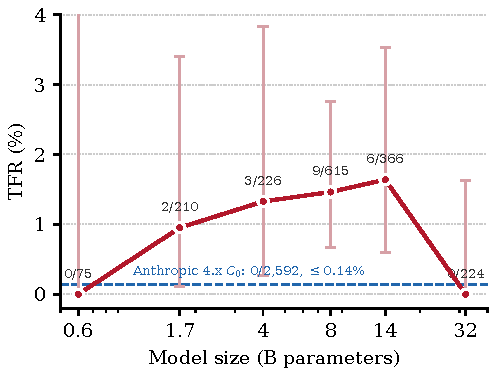
\includegraphics[width=0.98\linewidth]{figures/fig1_scaling_curve}
\caption{Qwen3-family tool-fabrication rate (TFR) under the opaque
baseline $\mathrm{C}_0$, four-distractor probe with the target tool
removed, $0.6$B--$32$B (per-call pooled; the same data as
Table~\ref{tab:qwen3-scale}). Points are pooled per-size TFR; error bars
are Clopper--Pearson $95\%$ intervals. The dashed line marks the pooled
Anthropic~4.x $\mathrm{C}_0$ upper bound ($0/2{,}592$, $\leq\!0.14\%$;
Section~\ref{sec:results:probe}), shown for reference. The shape is
non-monotone---near-zero at $0.6$B, a $\sim\!1$--$2\%$ band at $1.7$--$14$B,
and $0\%$ at $32$B---but with only six sizes and wide intervals (e.g.\ the
$32$B bound overlaps the $14$B estimate) we read it descriptively: a
single-family, single-quantization shape, \emph{not} a fitted scaling law
and \emph{not} evidence of an emergent capability. Quantization is held at
nominal $4$-bit across sizes but not at fixed reconstruction error per
checkpoint; we therefore do not attribute the shape to capability alone
(see Section~\ref{sec:limitations} and the bf16 control noted there).}
\label{fig:scaling}
\end{figure}

%      (or paste the figure environment below) at that point.
%   2. Update the in-body text reference: in 05_results.tex L102-103 change
%      "plotted in Appendix Figure~\ref{fig:scaling}" -> "plotted in
%      Figure~\ref{fig:scaling}" (drop the word "Appendix").
%   3. REMOVE the appendix copy: delete A1_appendix.tex L6-16 (the
%      \begin{figure}...\label{fig:scaling}...\end{figure} block) so the label
%      is defined exactly once and the figure is not duplicated.
%   4. The figure asset figures/fig1_scaling_curve.pdf is unchanged; only the
%      caption text below is updated (more descriptive, less overclaiming).
%
% NOTE on column width: \linewidth in a single-column ICML body figure spans
% one text column (~3.25in). fig1_scaling_curve.pdf was authored for the
% appendix at 0.8\linewidth; in-body, 0.95--1.0\linewidth reads better in one
% column. If the panel is too dense at column width, promote to a full-width
% figure with figure* and width=0.7\linewidth instead (costs more vertical
% space; only if the +1 page budget allows).
% =====================================================================

\begin{figure}[t]
\centering
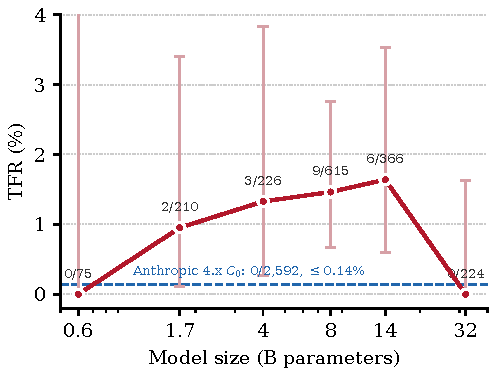
\includegraphics[width=0.98\linewidth]{figures/fig1_scaling_curve}
\caption{Qwen3-family tool-fabrication rate (TFR) under the opaque
baseline $\mathrm{C}_0$, four-distractor probe with the target tool
removed, $0.6$B--$32$B (per-call pooled; the same data as
Table~\ref{tab:qwen3-scale}). Points are pooled per-size TFR; error bars
are Clopper--Pearson $95\%$ intervals. The dashed line marks the pooled
Anthropic~4.x $\mathrm{C}_0$ upper bound ($0/2{,}578$, $\leq\!0.12\%$;
Section~\ref{sec:results:probe}), shown for reference. The shape is
non-monotone---near-zero at $0.6$B, a $\sim\!1$--$2\%$ band at $1.7$--$14$B,
and $0\%$ at $32$B---but with only six sizes and wide intervals (e.g.\ the
$32$B bound overlaps the $14$B estimate) we read it descriptively: a
single-family, single-quantization shape, \emph{not} a fitted scaling law
and \emph{not} evidence of an emergent capability. Quantization is held at
nominal $4$-bit across sizes but not at fixed reconstruction error per
checkpoint; we therefore do not attribute the shape to capability alone
(see Section~\ref{sec:limitations} and the bf16 control noted there).}
\label{fig:scaling}
\end{figure}
